
\chapter{Implementation}
The Implementation covers the process of implementing a localization system using orthogonal codes in underwater environments. It starts with the description of pulse shaping using a cosine FIR filter. Then, the signal is shifted to the carrier frequency of \SI{62.5}{\kilo\hertz}. To ensure the desired frequency characteristics, a band pass filter of 5th order Butterworth is applied. The signal is then shifted back to baseband, followed by a low-pass filter to remove any high-frequency components. The peak detection is performed using a CFAR (Constant False Alarm Rate) algorithm. Finally, the localization method is presented that uses the information obtained from peak detection to determine the position. 

The whole chain of processes, including pulse shaping, shift to carrier, band pass filtering, shift to baseband, low-pass filtering, peak detection, and the localization method, is implemented in Python.

\section{Pulse shaping}
The raw code which was previously generated is first put through an sign function, which sets its mean to zero. The discontinuous signal holds an infinite bandwidth because it consists of rectangular pulses. These pulse spans have infinity frequency, which are impossible to implement for acoustic transmission or at all. Therefore a restriction to a certain bandwidth must be introduced. Such a reduction is possible by applying an low-pass filter.

Because limiting the signals bandwidth introduces a damped oscillation, which leads to incorrect decoding of received data \cite{ken07}, a appropriate choice of filter would be a the raised cosine \ref{eq:cosfir}. Such a pulse filter is defined by a squared cosine, which decreases its amplitude in frequency. In our case the roll off factor $\alpha$ is set to $0.125$ and symbol length $T_{sym}$ to the inverse of our target bandwidth \SI{20}{\kilo\hertz}.

Before applying the filter the generated codes need to be up-scaled for our target sampling rate. The relation between sampling rate $f_s$ and up-sampling factor $Sp_s$ is $Sp_s=fs\cdot T_{sym}$.

\begin{equation}
	H(\omega)=T_{sym}\cdot \cos^2\left(\dfrac{T_{sym}(\omega-\pi(1-\alpha)/T_{sym})}{4\alpha}\right),~~~\omega=2\pi f
	\label{eq:cosfir}
\end{equation}


\begin{figure}[h]
	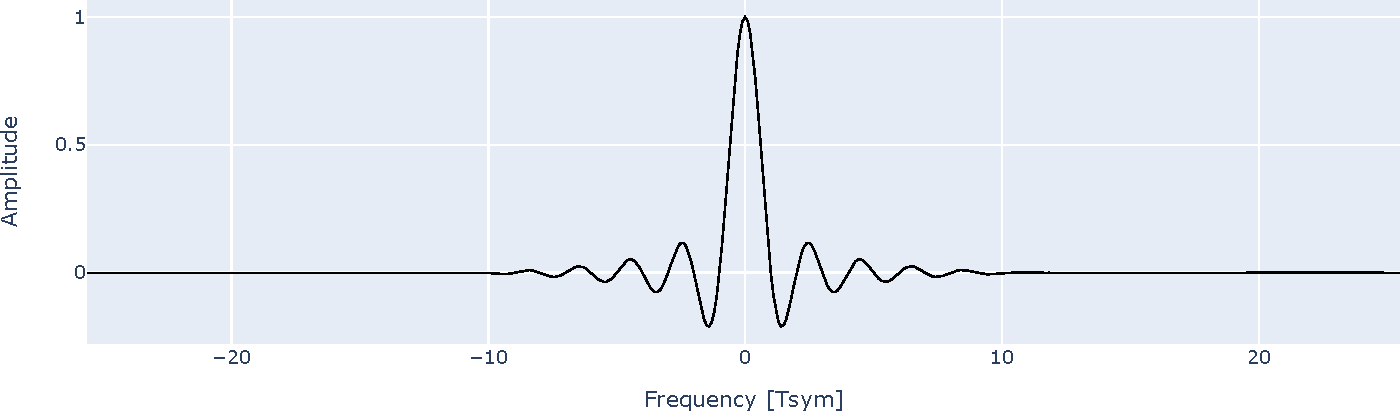
\includegraphics[width=\linewidth]{images/cosfir}
	\caption{Section of cosine FIR with a resolution of 1024}
	\label{fig:cosfir}
\end{figure}


\section{Shift to carrier}

Now that our base band signal $tSigBB[k]$ has its target bandwidth and sample rate only the frequency shift to the carrier frequency $f_c$ of \SI{62.5}{\kilo\hertz} is necessary. That procedure is accomplished by multiplying our sampled signal by the exponential function, where $f_c$ is passed to its exponent. An Frequency shift of the transmitted signal can be achieved by multiplying it with a complex exponential function of the form $e^{-2\pi j f_c k}$. This results in a phase rotation in the frequency domain and effectively shifts the spectrum of the signal by $f_c$. The resulting signal could hold imaginary parts, hence only the real part is passed through for transmission.

The signal is now in an almost appropriate state for the use inside an localization algorithm, where the delays of the signals can be detected by the help of cross-correlation techniques.
\begin{equation}
	x_{tSigTB}[k]=Re\{x_{tSigBB}[k]\cdot e^{-2\pi j f_c k}\}
	\label{eq:shift}
\end{equation}

%\begin{equation}
%	x_{tSigBB}[k]=x_{tSigTB}[k]\cdot e^{-2\pi j (-f_c) k}
%	\label{eq:rshift}
%\end{equation}

%\section{Simulation}
%The simulation consists of a watermark benchmark \cite{watermark15} and a additive GWN generated by a desired SNR between $-20dB$ and $20dB$ in steps of $5dB$. From the general equation of the Signal to Noise Ratio we derive our noise standard deviation by transforming this ratio. The white noise is added after the simulation and before receiver filtering.
%\begin{equation}
%	SNR=\cfrac{P_{Signal}}{P_{Noise}}=\cfrac{\mathbb{E}({Signal}^2)}{\mathbb{E}({Noise}^2)}=\cfrac{\sum {Signal}^2}{N\cdot\sigma_{Noise}^2}~~\Leftrightarrow~~\sigma_{Noise}=\sqrt{\cfrac{\sum^N {Signal}^2}{N\cdot SNR}}
%\end{equation}
%
%\begin{equation}
%	SNR_{dB}=10\cdot\log_{10}\cfrac{\sum Signal^2}{\sum Noise^2}
%	=10\left(\log_{10}\sum^N_{k=1} x_{TB}^2[k]-\log_{10}\sum^N_{k=1} Noise^2[k]\right)
%\end{equation}
%
%\begin{equation}
%	Noise=\text{\textsc{Normal}}(0,1)\cdot \cfrac{\sigma_{Signal}}{SNR}
%\end{equation}
\begin{figure}[h]
	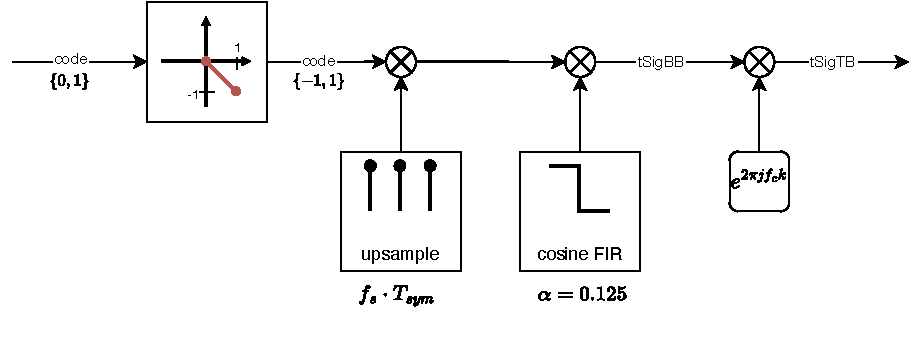
\includegraphics[width=\linewidth]{images/sensig}
	
	\caption{Processing of generated signal}
	\label{fig:sensig}
\end{figure}


\section{Band pass filter}
On the receiver side all signals are received as a sum, which is mixed by artifacts of signal reflections and random noise from the electronics.

The received signal may also have noise around its bandwidth because of its frequency shift. Thus, we only pass though frequencies inside our frequency band by applying a butterworth band pass filter.
A flat magnitude is favorable because only frequencies of the base-band should be passed through. 
The filter gets applied after shifting back to the base-band. Such a filter, namely a maximally flat magnitude filter, approximates this goal. The roll-off decreases by increasing the order of the system.

The critical frequencies of the applied filter are $f_c\pm\frac{bw}{2}$ by an Order of 5. Thus, frequencies get removed which are not inside the spectrum of interest. To remove shifts in time the filter is applied forwards and backwards following a doubling of its order.
\section{Shift to base band}

Shifting the transmitted signal back to its original frequency is feasible by just changing the sign of $f_c$. In this case also the imaginary part can be retained.

\begin{equation}
	x_{tSigBB}[k]=x_{tSigTB}[k]\cdot e^{2\pi j f_c k}
	\label{eq:rshift}
\end{equation}
\section{Low-pass filter}
Due to the presence of residuals within the transfer-band originating from the product of frequency shift, a low-pass filter was utilized. This filter is a Butterworth filter, which had previously been employed by the same order. Additionally, the filter is applied in both forward and backward directions, thereby eliminating any time shift.
\begin{figure}[h]
	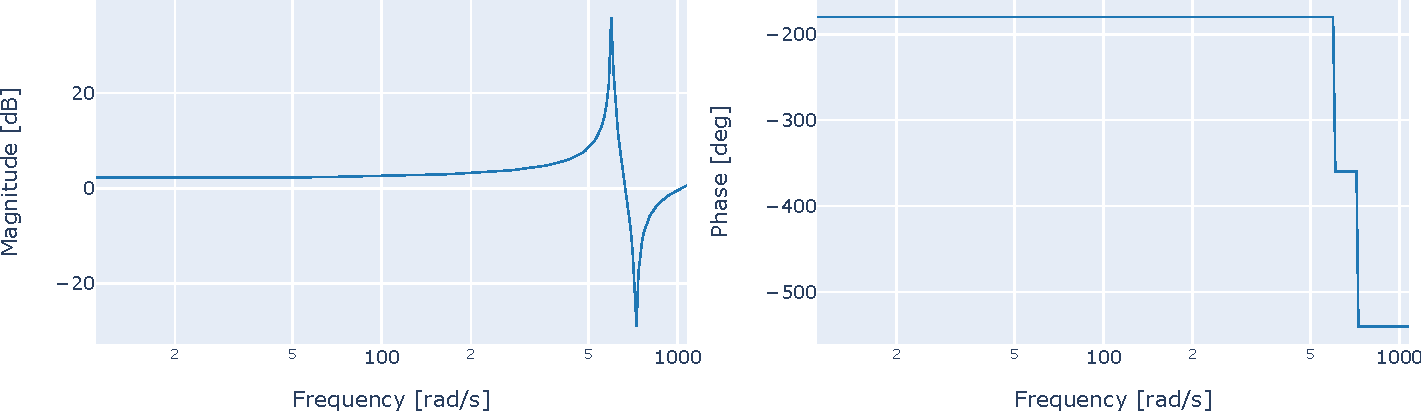
\includegraphics[width=\linewidth]{images/bode}
	
	\caption{Bode plot of 5th order Butterworth low-pass filter}
	\label{fig:bode}
\end{figure}
\begin{figure}[h]
	\centering
	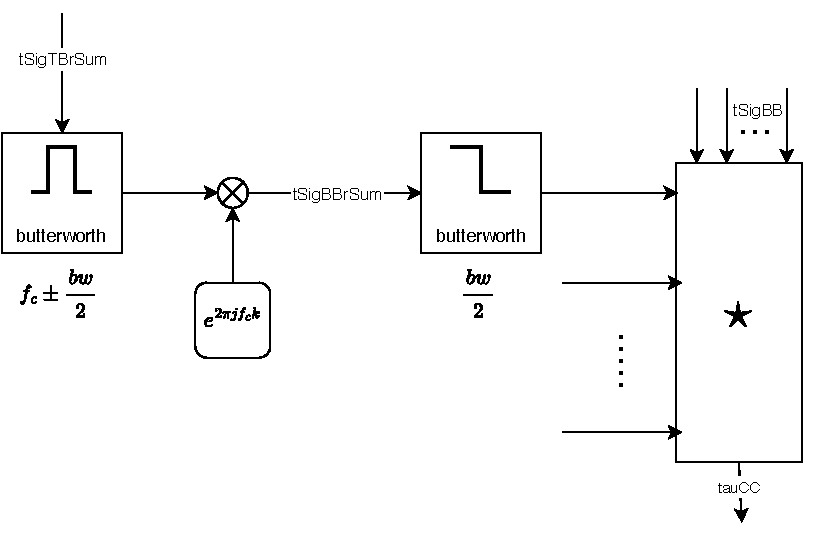
\includegraphics[width=\linewidth]{images/recsig}
	\caption{Processing of received signal}
	\label{fig:recsig}
\end{figure}

\section{Peak detection}

The received signal, consisting of summed delayed signals, cross-correlated by every anchor. If the signal is not reflected the peak in cross-correlation would be obvious. But by the introduction of noise and water reflections a higher rate of similar peaks appear. To suppress these effects a CFAR Algorithm \cite{rohling11} is applied to only detect the first reflected peak resulting in lower false alarms of peaks.

CFAR works by using multiple values intervals. The most outer one could be described as a train bin and is used to get an estimation of the signals noise. Especially CA-CFAR (cell-averaging constant false alarm rate) uses averaging to estimate the noise by measured cells. The bordering bin, defined as the guard cells, is used to reduce self-interference of the peaks. Thus, increasing window sizes $W$ results in better noise estimating but overall detectability is still limited by the sample rate  \cite{rohling11}\cite{radarbasics}. By knowledge of measured peak widths a optimal guard interval can be figured.

The calculated threshold is than scaled by factor $S$ depending on a formula based on the false alarm rate $\eta$. The higher the false alarm rate, the weaker high amplitude peaks gets included by the estimated threshold \ref{eq:cff}.\\

%Because Cell Averaging shows not satisfactory results in sensitive multi targets examples, the noise estimation could be enhanced by a sorting average applied to the %train interval. That principle is defined as CO-FAR \cite{rohling11}. 
%\begin{center}
%	\begin{tabular}{|c|c|}
	%			\hline
	%			candidate sample & $i$\\
	%			\hline
	%			guard interval (half) & $\mathcal{G}$ \\
	%			\hline
	%			train interval (half) & $\mathcal{T}$ \\
	%			\hline
	%			false alarm rate & $\eta$\\
	%			\hline
	%		\end{tabular}
%	\linebreak
%\end{center}
%
%\begin{equation}
%	Threshold(i)_x=
%	\cfrac{\alpha}{2\mathcal{T}}
%	\left[ \sum_{j=i-\left( \mathcal{G}+\mathcal{T}\right) }^{i+\left( \mathcal{G}+\mathcal{T}\right)}x(j) - \sum_{j=i-\mathcal{G}}^{i+\mathcal{G}}x(j) \rigbest NAht] 
%	\label{eq:cft}
%\end{equation}
\begin{equation}
	S=2W\left( \eta^{-1/{2W}}-1\right) 
	\label{eq:cff}
\end{equation}

\begin{figure}[!h]
	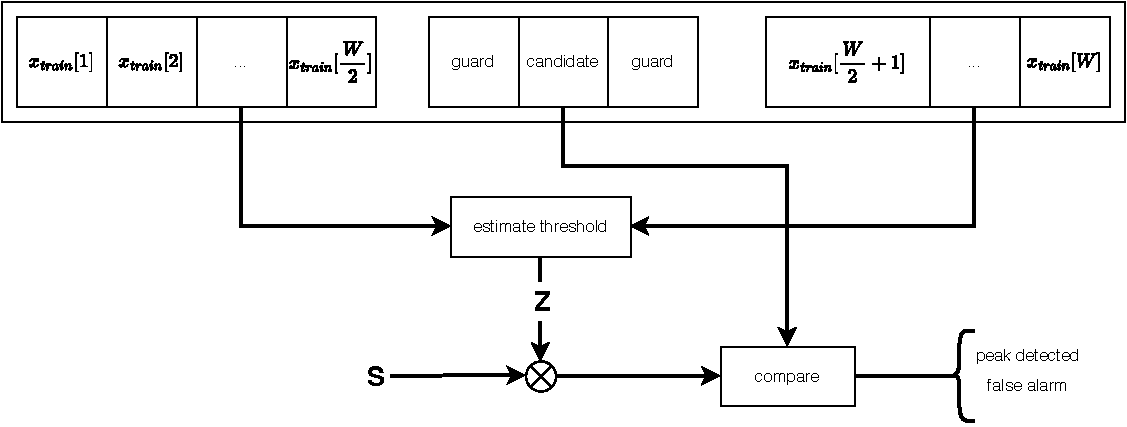
\includegraphics[width=\linewidth]{images/peakdet}
	
	\caption{CFAR threshold peak detection procedure \cite{rohling11}}
	\label{fig:simsig}
\end{figure}

\begin{equation}
	T=S\cdot Z,~~~Z_{CA}=\sum_{i=1}^{W}\dfrac{1}{W}x_{train}
\end{equation}
%\section{Explicit Position calculation}
%
%The initial condition for the localization are four anchors $S_i$ with thir coordinates $\{x_i,y_i,z_i\}$ and the target $S$ which is to be located. By multiplying relative delays by the speed of sound $c$ which is approximately set to $1500\,\frac{m}{s}$, the distance $d_{ij}$ between the reference anchor $S_0$ and $S_i$ is calculated.\\
%\begin{equation}
%	d_{ij}=c\cdot\tau_{ij}=c\cdot (t_i-t_j),~~~\text{absolute delays } t_k,~k\in \{0,1,2,3\}
%\end{equation}
%By these values a Matrix $A$ and vector $\vec{b}$ is created. Thus, a System $A\cdot \vec{x}=\vec{b}$ is established. This linear system can be solved by using the inverse method if Matrix $A$ has full rank. Otherwise least squared can be used but yields undesirable results. In three dimensional Space five anchors are needed for full rank. The solution $\vec{x}$ are the coordinates $\{x,y,z\}$ of the target $S$ \cite{yang11}.
%
%\begin{equation}
%	A=\left[
%	\begin{array}{cccc}
	%		x_0-x_1 & y_0-y_1 & z_0-z_1 & d_{01}\\
	%		x_0-x_2 & y_0-y_2 & z_0-z_2 & d_{02}\\
	%		x_0-x_3 & y_0-y_3 & z_0-z_3 & d_{03}\\
	%		x_0-x_4 & y_0-y_4 & z_0-z_4 & d_{04}\\
	%	\end{array}
%	\right]
%\end{equation}
%\begin{equation}
%	\vec{b}=\cfrac{1}{2}\left[
%	\begin{array}{c}
	%		x_0^2-x_1^2+y_0^2-y_1^2+z_0^2-z_1^2+d_{01}^2\\
	%		x_0^2-x_2^2+y_0^2-y_2^2+z_0^2-z_2^2+d_{02}^2\\
	%		x_0^2-x_3^2+y_0^2-y_3^2+z_0^2-z_3^2+d_{03}^2\\
	%		x_0^2-x_4^2+y_0^2-y_4^2+z_0^2-z_4^2+d_{04}^2\\
	%	\end{array}
%	\right]
%	,~~~
%	\vec{x}=\left[
%	\begin{array}{c}
	%		x\\
	%		y\\
	%		z\\
	%		||S-S_0||_2\\
	%	\end{array}
%	\right]
%\end{equation}
%Theoretically an system $A$ of lower rank can be solve by least squares. Having said this, positions calculated by that approach could not satisfy the demands of 3D localization.
%
%\begin{equation}
%	\vec{x}=(A^T A)^{-1} A^T\vec{b}
%\end{equation}

\section{Localization method}

The initial condition for the localization are four anchors $S_i$ with thir coordinates $\{x_i,y_i,z_i\}$ and the target $S$ which is to be located. By multiplying relative delays by the speed of sound $c$ which is approximately set to \SI{1500}{\meter\per\second}, the distance $d_{ij}$ between the reference anchor $S_0$ and $S_i$ is calculated  \cite{yang11}.

\begin{equation}
	d_{ij}=c\cdot\tau_{ij}=c\cdot (t_i-t_j),~~~\text{absolute delays } t_k,~k\in \{0,1,2,3\}
\end{equation}
\begin{equation}
	x_{ji}:=x_j-x_i,~~~~~
	y_{ji}:=y_j-y_i,~~~~~
	z_{ji}:=z_j-z_i~~~~~
\end{equation}
Every TDOA estimate creates hyperbolic curves which anchors is placed at its foci. 
By rearranging the derivation of hyperbola intersections the following substitutes can be defined \cite{bucher02}. 

\begin{equation}
	{A}=\cfrac{d_{02}x_{10}-d_{01}x_{20}}{d_{01}y_{20}-d_{02}y_{10}},~~~
	{B}=\cfrac{d_{02}z_{10}-d_{01}z_{20}}{d_{01}y_{20}-d_{02}y_{10}}
\end{equation}	
(See appendix for complete formula)

%\begin{equation}
%	{C}=\cfrac{d_{02}\left(d_{01}^2+x_0^2-x_1^2+y_0^2-y_1^2+z_0^2-z_1^2\right)-d_{01}\left(d_{02}^2+x_0^2-x_2^2+y_0^2-y_2^2+z_0^2-z_2^2\right)}{2\left(d_{01}y_{20}-d_{02}y_{10}\right)}
%\end{equation}	
%
%\begin{equation}
%	{D}=\cfrac{d_{23}x_{12}-d_{21}x_{32}}{d_{21}y_{32}-d_{23}y_{12}},~~~
%	{E}=\cfrac{d_{23}z_{12}-d_{21}z_{32}}{d_{21}y_{32}-d_{23}y_{12}}
%\end{equation}	
%\begin{equation}
%	{F}=\cfrac{d_{23}\left(d_{21}^2+x_1^2-x_1^2+y_1^2-y_1^2+z_0^2-z_1^2\right)-d_{21}\left(d_{23}^2+x_1^2-x_2^2+y_1^2-y_2^2+z_1^2-z_2^2\right)}{2\left(d_{21}y_{32}-d_{23}y_{12}\right)}
%\end{equation}	
%
%\begin{equation}
%	{G}=\cfrac{{E}-{B}}{{A}-{D}},~~~
%	{H}=\cfrac{{F}-{C}}{{A}-{D}},~~~
%	{I}={A}\cdot {G}+{B},~~~
%	{J}={A}\cdot {H}+{C}
%\end{equation}	
%
%\begin{equation}
%	{K}=d_{02}^2+x_0^2-x_2^2+y_0^2-y_2^2+z_0^2-z_2^2+2x_{20}{H}+2y_{20}{J}
%\end{equation}	
%
%\begin{equation}
%	{L}=2\left(x_{20}{G}+y_{20}{I}+z_{20}\right)
%\end{equation}	
%
%\begin{equation}
%	{M}=4d_{02}^2\left({G}^2+{I}^2+1\right)-{L}^2
%\end{equation}	
%
%\begin{equation}
%	{N}=8d_{02}^2\left[{G}\left(x_0-{H}\right)+{I}\left(y_0-{J}\right)+z_0\right]+2{L}\cdot{K}
%\end{equation}	
%
%\begin{equation}
%	{O}=4d_{02}^2\left[\left(x_0-{H}\right)^2+\left(y_0-{J}\right)^2+z_0^2\right]-{K}^2
%\end{equation}	
A downside of this approach is the uncertainty of position $z$. Thus, additional information on bounds is necessary. The target won't get above sea level. Consequently, at least one boundary $z_{surface}$ which acts like a maximum can be set. The minimum value $z_{ground}$ can be assumed as the lowest position achievable underwater. 
\begin{equation}
	z_{a,b}=\cfrac{{N}}{2{M}}\pm\sqrt{\left(\cfrac{{N}}{2{M}}\right)^2-\cfrac{{O}}{{M}}}
\end{equation}	

\begin{equation}
	z=\min\left\{\max\left\{z_a,~z_b,~z_{surface}\right\},~z_{ground}\right\}
\end{equation}	

One other solution to this issue is to utilize information about our previous location $z'$. Specifically, we can calculate the distance between our current position and the two potential candidates for the next estimate of $z$, and choose the candidate with the shorter distance.
\begin{equation}
	z=\begin{cases}
		z_a & \text{if }\abs{z_a-z'}<\abs{z_b-z'}\\
		z_b & \text{else}
	\end{cases}
\end{equation}	

The resulting $x$ and $y$ values of our target can then be calculated by the following formula using the selected $z$, completing the desired position vector $\vec{x}$.
\begin{equation}
	\vec{x}
	=\left[
	\begin{array}{c}
		x\\
		y\\
		z
	\end{array}
	\right]
	=\left[
	\begin{array}{c}
		{G}z+{J}\\
		{I}z+{H}\\
		z
	\end{array}
	\right]
\end{equation}	